\documentclass[a4paper]{article}
\usepackage{MMVII}

\newcommand{\TheCmd}{VisuPose3D}

\begin{document}

\CmdTitle
%\maketitle

\tableofcontents

 %=================================================================================

\SecDescr

This command create   a $3d$ visualisation of poses  and also, possibly,
a sparse visualisation of the scene (using tie points).
The visualisation is made using point cloud in ply format because it can be
read very easily on various free open source software.

The poses of camera are visualized using a pyramid for rectilinear camera and 
set of "meridian" for fisheye or lidar station (see ~\ref{fig:VisuPose3D} , a picture is worth a thousand words).


 %=================================================================================

\section{fixing size of pyramid}

The size of the pyramid is proportionnal to the $35mm$ focal length
(precisely the focal in pixel divided by diagonal of image). 

The default rule to compute this degree of proportionnality uses the
parameter \FileSty{ELPFD} \footnote{Evaluate Lenght Pyramid From Depth \dots} 
and the tie points :


\begin{itemize}
   \item  a depth $D$ is computed using a proportion of  all the depth of all tie points (default $30\%$);
   \item  this depth $D$ is mutilpied by a factor (default $\frac{1}{10}$).
\end{itemize}

If the value of parameter \FileSty{CamScale} is set it is used 
instead of the previous computation.  The default value of   \FileSty{CamScale} ($\frac{1}{10}$)  is also
used if there is no tie-points .


\begin{figure}
\centering
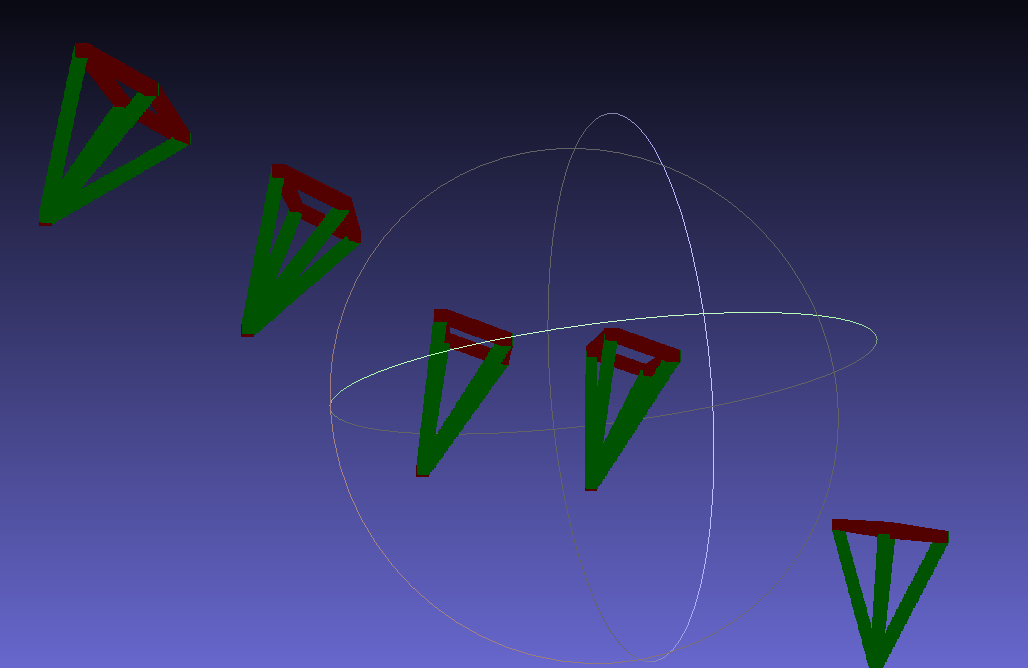
\includegraphics[width=6cm]{Images/VisuPose3D-RectiLinear.png}
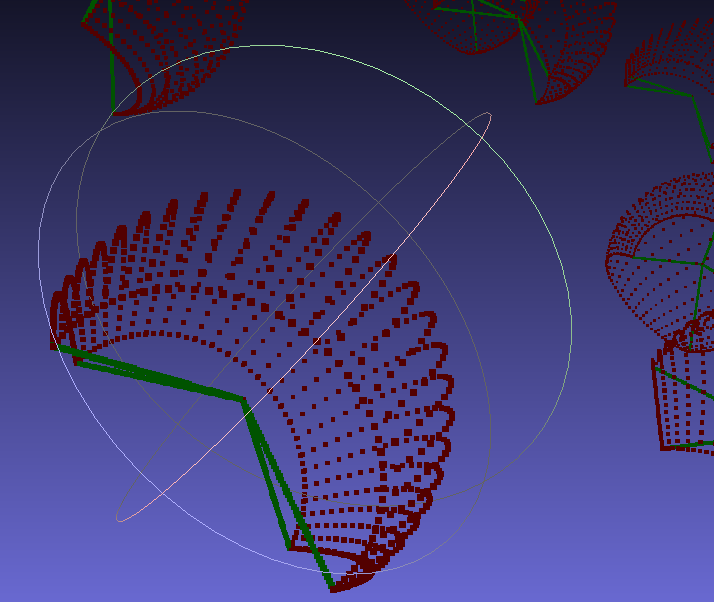
\includegraphics[width=6cm]{Images/VisuPose3D-FishEye.png}
        \caption{Result of \TheCmd with "standard" camera and fisheye}
        \label{fig:VisuPose3D}
\end{figure}





\end{document}
